\documentclass[12pt]{article}
\usepackage{letltxmacro}
\usepackage{makeidx}
\usepackage{multirow}
\usepackage{multicol}
\usepackage[dvipsnames,svgnames,table]{xcolor}
\usepackage{graphicx}
\usepackage{epstopdf}
\usepackage{ulem}
\usepackage{hyperref}
\usepackage{amsmath}
\usepackage{amssymb}
\usepackage{lipsum}
\usepackage{setspace}
%\usepackage{fontspec}
%\usepackage[T1]{fontenc}
%\usepackage[utf8]{inputenc}
%\usepackage{mathptmx}
%\setmainfont{Times New Roman}
\title{}
\usepackage[paperwidth=595pt,paperheight=841pt,top=72pt,right=72pt,bottom=72pt,left=72pt]{geometry}

\makeatletter
	\newenvironment{indentation}[3]%
	{\par\setlength{\parindent}{#3}
	\setlength{\leftmargin}{#1}       \setlength{\rightmargin}{#1}%
	\advance\linewidth -\leftmargin       \advance\linewidth -\rightmargin%
	\advance\@totalleftmargin\leftmargin  \@setpar{{\@@par}}%
	\parshape 1\@totalleftmargin \linewidth\ignorespaces}{\par}%
\makeatother 

% new LaTeX commands
\renewcommand{\baselinestretch}{1.5} 
\renewcommand*{\familydefault}{\rmdefault}
\begin{document}

\pagenumbering{gobble}
\begin{center}
\begin{indentation}{0pt}{0pt}{0pt}
\vspace{10cm}
\textbf{{\Large AN SDN APPROACH FOR EFFICIENT INTERNET BANDWIDTH UTILIZATION IN WIRELESS MESH NETWORKS}}
\end{indentation}
\end{center}

\vspace{0.5cm}

\begin{center}
\begin{indentation}{0pt}{0pt}{0pt}
{\large{\textbf {\textit {Submitted by}}}}
\end{indentation}
\end{center}
\vspace{0.5cm}

\begin{center}
\begin{indentation}{0pt}{0pt}{0pt}
{\large \bf ASHISH GUPTA}
\end{indentation}
\end{center}

\begin{center}
\begin{indentation}{0pt}{0pt}{0pt}
{\large \bf CHANDRIKA PARIMOO}
\end{indentation}
\end{center}

\begin{center}
\begin{indentation}{0pt}{0pt}{0pt}
{\large \bf RUTUJA SHAH}
\end{indentation}
\end{center}

\begin{center}
\begin{indentation}{0pt}{0pt}{0pt}
{\large \bf SUDIPTO CHATTERJEE}
\end{indentation}
\end{center}
\vspace{1cm}

\begin{center}
\begin{indentation}{0pt}{0pt}{0pt}
{\large \bf Pune Institute of Computer Technology}
\end{indentation}
\end{center}

\begin{center}
\begin{indentation}{0pt}{0pt}{0pt}
{\large \bf Team ID:QPP1003}
\end{indentation}
\end{center}
\pagebreak

\begin{indentation}{0pt}{0pt}{0pt}
\textbf{{{\Large Abstract}}}
\end{indentation}
\vspace{0.5cm}
\begin{indentation}{0pt}{0pt}{0pt}
{\normalsize \hspace{1cm} Wireless Mesh Networks(WMN) have been emerging in the last couple of years as a cost effective alternative to traditional wired access networks. A typical WMN combines a fixed network (backbone) and a mobile network (backhaul). The nodes in a WMN often act as relays, forwarding traffic to or from other mesh nodes, or providing localized connectivity to mobile or pervasive wireless devices, such as laptops, desktops and other mobile clients. Some of these nodes, called mesh gates, act as gateways that are directly connected to the Internet. Among the various variants of mesh networks, IEEE 802.11s is the IEEE standard for Wireless Mesh Networks and is also present in the Linux kernel. This project uses o11s (open80211s), which is the implementation of IEEE 802.11s in the Linux kernel, as the underlying mesh network.}
\end{indentation}

\begin{indentation}{0pt}{0pt}{0pt}
{\normalsize \hspace{1cm}Currently, in o11s, every mesh node is associated with a maximum of one mesh gate. This type of single association involves the entire traffic being directed towards the mesh gate. The gate's available bandwidth is shared by all its clients, and consequently, the throughput per client is reduced with an increase in the number of clients. Additionally, constraints such as the mesh gate being common to many outbound paths reduce the effective link capacity due to the multipoint-to-point nature of the traffic.}
\end{indentation}
\begin{indentation}{0pt}{0pt}{0pt}
{\normalsize \hspace{1cm}This project aims to improve the utilization of total available bandwidth by using multiple Internet access gateways inside a Wireless Mesh Network instead of the usual association with a single Internet gateway. This is achieved transparently without any changes to applications using the mesh. Traffic sensitive load sharing is also incorporated for the selection of gateways.}
\end{indentation}

\begin{indentation}{0pt}{0pt}{0pt}
{\normalsize \hspace{1cm}The benefits include increased network throughput as well as reduced network setup costs as the need for additional network hardware is eliminated.}
\end{indentation}

\begin{indentation}{0pt}{0pt}{0pt}
\vspace{1cm}
\textbf{{{\Large Problem Statement}}}
\end{indentation}
\vspace{0.5cm}

\begin{indentation}{0pt}{0pt}{0pt}
{\normalsize \hspace{1cm} Enhance bandwidth utilization in Wireless Mesh Networks using a decentralized approach to improve throughput.}
\end{indentation}

\begin{indentation}{0pt}{0pt}{0pt}
  \vspace{1cm}
 \pagebreak
\textbf{{{\Large Solution}}}
\end{indentation}
\vspace{0.5cm}
\begin{indentation}{0pt}{0pt}{0pt}
{\normalsize \hspace{1cm} The devised solution makes use of all gateways present in the Wireless Mesh Network. The packets are categorized on a per flow basis and not on a per packet basis as it helps us not worry about deep packet inspection in order to determine the correct path. Since a single flow of packets is categorized by open ports in the sender as well as the receiver, we use the source port on the sender as a unique key for relating to a specific flow. This helps preserve the sanity of applications as well as meet their expectations of seeing all packets of the same flow on the same port.}
\end{indentation}


\begin{indentation}{0pt}{0pt}{0pt}
  {\normalsize \hspace{1cm} A gate is a machine which is connected to the mesh network using a wireless interface and has an internet connection available on another interface. Both these interfaces are bridged in order to make use of both the mesh capabilities as well as the Internet capabilities simultaneously. The gate broadcasts it's ability to perform as a gate by periodically sending out L2 packets containing it's IP address among other metrics. Traffic originating within the mesh network which is destined for an external network is routed using one of the available gates. The gateway is selected based on metrics such as the hop count and available link capacity. Traffic destined for the local network is not routed through the gate, and never leaves the local network.} 
\end{indentation}

\begin{indentation}{0pt}{0pt}{0pt}
{\normalsize \hspace{1cm}While the total and available bandwidth help in deciding the load on the mesh gate, the latency which also takes into account the hop count while routing to the gateway is a critical factor in routing http and VoIP traffic. Network capacity can increase linearly with the number of gateways only with proper load balancing and resource provisioning. This kind of proper association, which prevents the formation of bottlenecks and distributes the network load evenly realizes the linear capacity increase.}
\end{indentation}


\begin{indentation}{0pt}{0pt}{0pt}
{\normalsize \hspace{1cm} Through experimental setups using Click modular router it is demonstrable that unless the underlying hardware link capacity becomes the bottleneck, linear gain in the network takes place.}
\end{indentation}

\begin{figure}[t]
  \centering
    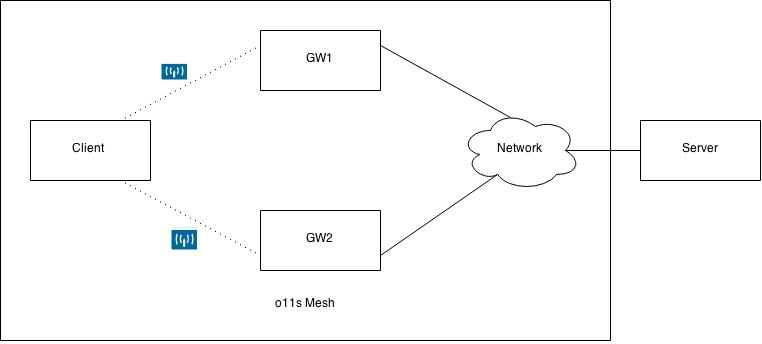
\includegraphics[scale=0.50]{ExperimentLayout}
    \caption{Experiment to show linear gain in the network.}
    \label{Diagram: Experiment layout}
\end{figure}
\vspace*{1cm}
\begin{figure}[b]
    \centering
    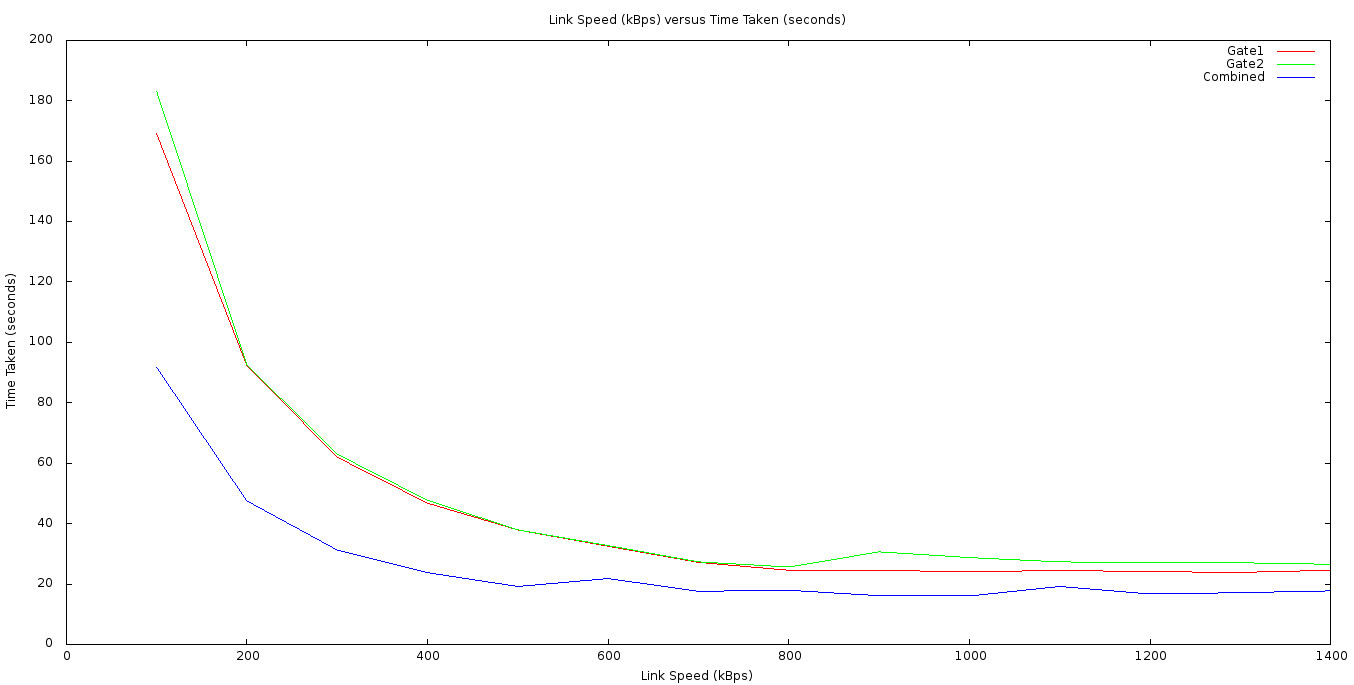
\includegraphics[scale=0.35]{ExperimentGraph}
    \caption{Results of the experiment.}
    \label{Graph: Result}
\end{figure}

%\pagebreak
\begin{indentation}{0pt}{0pt}{0pt}
\textbf{{{\Large Result and Discussion}}}
\end{indentation}
\vspace{0.5cm}

\begin{indentation}{0pt}{0pt}{0pt}
  {\normalsize \hspace{1cm} The diagram above shows the layout of the machines used for the experiment. The link capacities on either sides of both GW1 and GW2 are kept identical and varied from 100 KBPS to 1400 KBPS. Downloads were performed for each value of link speed once with GW1, once with GW2 and once with GW1 and GW2 simultaenously. The graph below was created with experimental readings and it clearly shows  gain in the network when download times are considered. Starting with a linear fashion, the gains become constant as the link speed approaches the link speed of the underlying hardware link.}
\end{indentation}

\begin{indentation}{0pt}{0pt}{0pt}
{\normalsize \hspace{1cm} Scenarios in which the number and type of gates keep changing such as a fluid mesh created due to the interaction of several mobile devices require special attention and demand to be handled as a part of the solution. In the case where a mesh gate is added to the network, the nodes should be able to make use of the new capabilities as soon as possible. Although it seems fairly straightforward to accommodate a new gate, the problem is that some flows which were mapped previously to the gateways that already existed may get mapped to the new gateway during a transaction. This will lead to a loss of data as the machine present on the other side of the gateways does not recognize the new gateway and will simply drop the packets as they are sent. For this, a mechanism to cache and to "remember" which flows are mapped to which gateways is required. This cache can simply forget about the association after terminal packets such as a TCP FIN in case of TCP connections are detected. This approach makes possible the addition of gates dynamically without resulting in packet loss for the existing network.}
\end{indentation}

\begin{indentation}{0pt}{0pt}{0pt}
{\normalsize \hspace{1cm} Regarding the situation where a mesh gate may go down owing to hardware failure or network failure, the solution aims to find an alternate route through which the packets must be routed. The packets that were transmitted to the failed gate earlier will of course require retransmission which can be achieved using a TCP Reset packet in most scenarios. In other scenarios, the only option may be to open a new socket and retransmit the whole stream once again.}
\end{indentation}


\begin{indentation}{0pt}{0pt}{0pt}
\vspace{1cm}
\textbf{{{\Large Practical Applications}}}
\end{indentation}
\vspace{0.5cm}

\begin{indentation}{0pt}{0pt}{0pt}
{\normalsize \hspace{1cm} Wherever more than one internet access point is available, the solution will help users achieve a higher network throughput. The gains will be visible in browsing for HTTP traffic. Although the user may not feel the effects at a small scale where less transactions are involved. Downloading big files over HTTP using multiple ranged-byte http requests using multiple connections will result in faster download times. Bittorrent, as it acquires data from multiple peers and uses multiple flows also benefits from this scheme. As the solution is at the L3/L2 of the OSI Network model, it is transparent to most applications and they should work without any changes to their code base.}
\end{indentation}

\begin{indentation}{0pt}{0pt}{0pt}
\vspace{1cm}
\textbf{{{\Large Summary}}}
\end{indentation}
\vspace{0.5cm}

\begin{indentation}{0pt}{0pt}{0pt}
{\normalsize \hspace{1cm} The sole aim of this project has been to achieve faster speeds for users while at the same time, being transparent to applications at higher layers. Various scenarios have been tested and experiments conducted as a proof of concept. These experiments have also been extended to real life scenarios where gain is visible.}
\end{indentation}

\end{document}
